\documentclass[border=10pt]{standalone}
\usepackage[T1]{fontenc}
\usepackage[utf8]{inputenc}
\usepackage{circuitikz}
\usepackage{amsmath,amssymb}
\usetikzlibrary{positioning,calc}
\ctikzset{bipoles/length=1.1cm, font=\small}

\definecolor{fondo}{HTML}{0B0F17}
\definecolor{tinta}{HTML}{E2E8F0}
\definecolor{ambar}{HTML}{FB923C}
\definecolor{cyan}{HTML}{38BDF8}
\definecolor{verde}{HTML}{4ADE80}
\definecolor{rojo}{HTML}{F87171}
\definecolor{gris}{HTML}{64748B}

\begin{document}
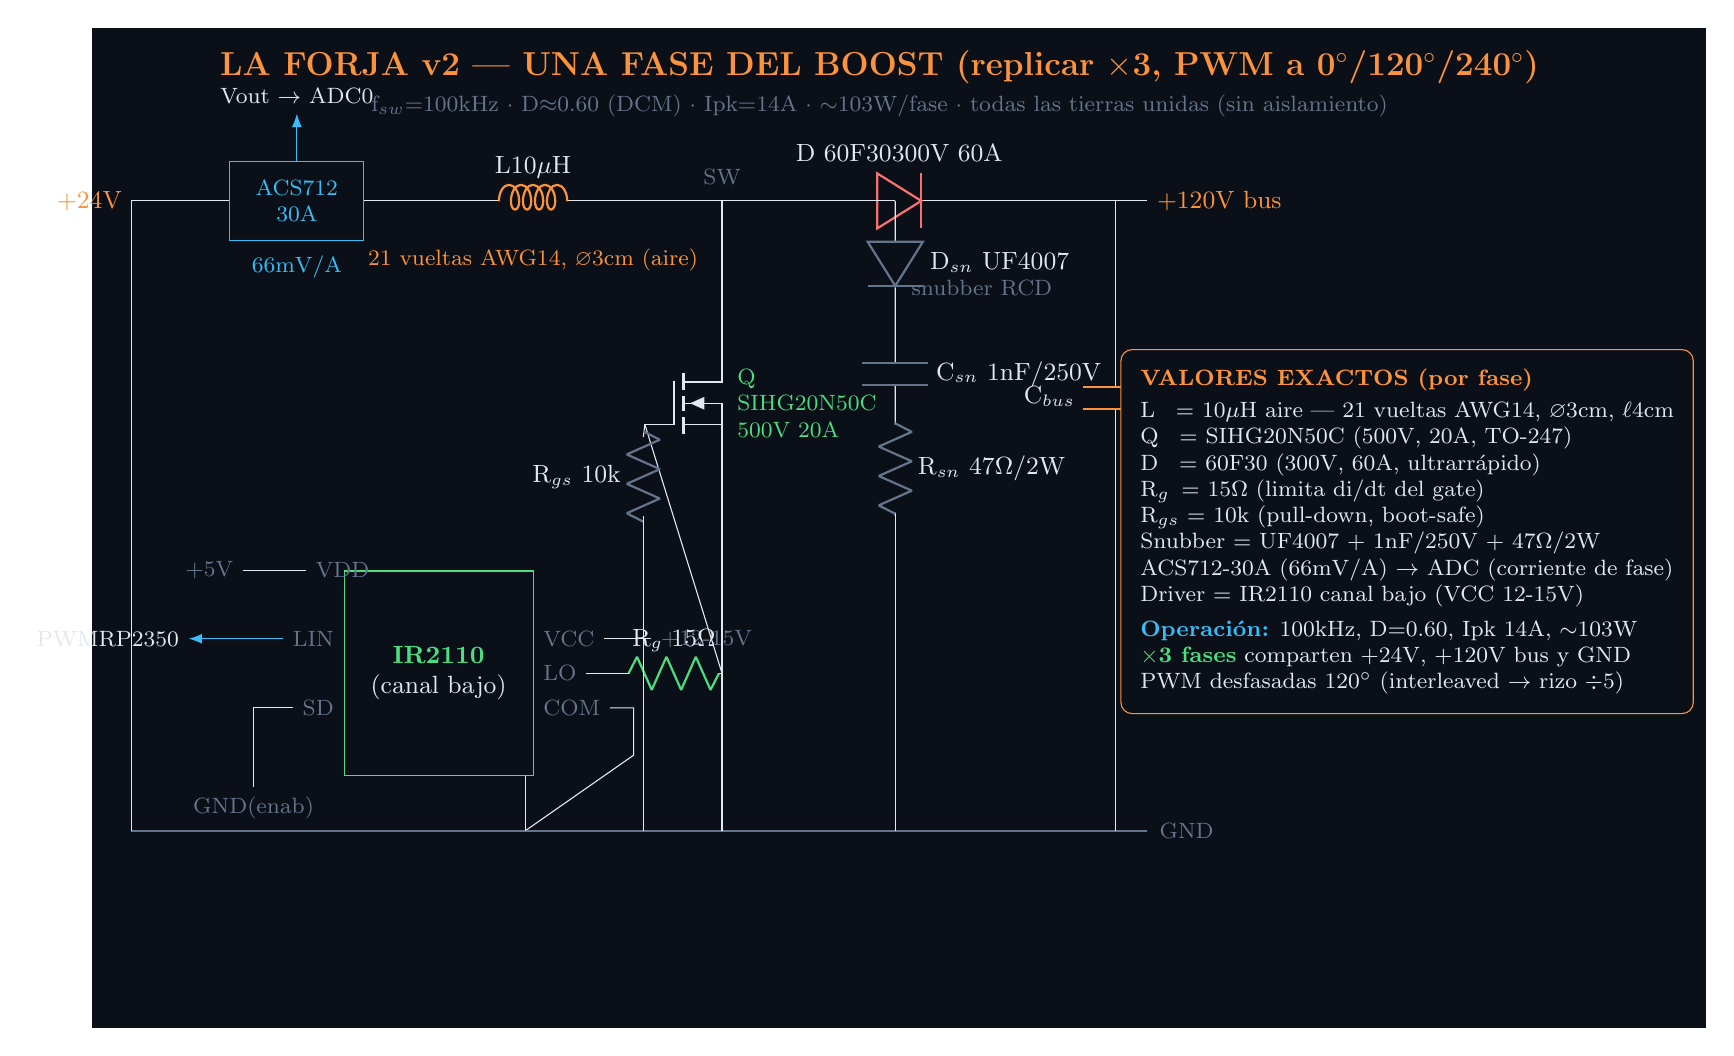
\begin{tikzpicture}[font=\small, every node/.style={text=tinta}]
\fill[fondo] (-3,-8.5) rectangle (17.5,4.2);

\node[text=ambar, font=\bfseries\large] at (7,3.7) {LA FORJA v2 — UNA FASE DEL BOOST (replicar $\times$3, PWM a 0$^\circ$/120$^\circ$/240$^\circ$)};
\node[text=gris, font=\footnotesize] at (7,3.2) {f$_{sw}$=100kHz $\cdot$ D$\approx$0.60 (DCM) $\cdot$ Ipk=14A $\cdot$ $\sim$103W/fase $\cdot$ todas las tierras unidas (sin aislamiento)};

\begin{scope}[color=tinta]

% ================= camino de potencia =================
% riel +24V
\draw (-2.5,2) node[left,text=ambar]{+24V} -- (-1.6,2);
% ACS712 (sensor de corriente de fase)
\node[draw=cyan, fill=fondo, text=cyan, minimum width=1.7cm, minimum height=1.0cm, align=center, font=\footnotesize] (acs) at (-0.4,2) {ACS712\\30A};
\draw (-1.6,2) -- (acs.west);
\draw (acs.east) -- (1.2,2);
\node[text=cyan, font=\footnotesize, below=2pt of acs] {66mV/A};
\draw[cyan,-{Latex}] (acs.north) -- ++(0,0.6) node[above,font=\footnotesize]{Vout $\to$ ADC0};

% bobina de aire
\draw (1.2,2) to[L, l=L\\10$\mu$H, color=ambar] (4.0,2);
\node[text=ambar, font=\footnotesize] at (2.6,1.25) {21 vueltas AWG14, $\varnothing$3cm (aire)};
% nodo SW
\draw (4.0,2) -- (5.0,2) coordinate(sw);
\node[text=gris,font=\footnotesize] at (5.0,2.3) {SW};

% diodo al bus
\draw (sw) to[D, l=D 60F30\\300V 60A, color=rojo] (9.5,2);
\draw (9.5,2) -- (10.4,2) node[right,text=ambar]{+120V bus};
% cap de bus (referencia)
\draw (10.0,2) to[C, l_={C$_{bus}$}, color=ambar] (10.0,-3);

% MOSFET Q (low-side)
\node[nigfete, anchor=D] (Q) at (5.0,0.2) {};
\draw (sw) -- (Q.D);
\node[text=verde, font=\footnotesize, right=2pt of Q, align=left] {Q\\SIHG20N50C\\500V 20A};
% source a GND
\draw (Q.S) -- (5.0,-2);

% snubber RCD a traves del MOSFET (SW->GND)
\draw (sw) ++(0.0,0) -- (7.2,2);
\draw (7.2,2) to[D, l=D$_{sn}$ UF4007, color=gris] (7.2,0.4);
\draw (7.2,0.4) to[C, l=C$_{sn}$ 1nF/250V, color=gris] (7.2,-0.8);
\draw (7.2,-0.8) to[R, l=R$_{sn}$ 47$\Omega$/2W, color=gris] (7.2,-2);
\node[text=gris,font=\footnotesize] at (8.3,0.9) {snubber RCD};

% ================= gate drive (IR2110) =================
\node[draw=verde, fill=fondo, text=tinta, minimum width=2.4cm, minimum height=2.6cm, align=center] (drv) at (1.4,-4) {\textbf{\textcolor{verde}{IR2110}}\\(canal bajo)};
% pines
\node[text=gris,font=\footnotesize,left=0pt of drv.160] (lin) {LIN};
\node[text=gris,font=\footnotesize,left=0pt of drv.200] (sd) {SD};
\node[text=gris,font=\footnotesize,left=0pt of drv.120] (vdd) {VDD};
\node[text=gris,font=\footnotesize,right=0pt of drv.20] (vcc) {VCC};
\node[text=gris,font=\footnotesize,right=0pt of drv.0] (lo) {LO};
\node[text=gris,font=\footnotesize,right=0pt of drv.-20] (com) {COM};
% conexiones del driver
\draw[cyan,-{Latex}] (lin.west) -- ++(-1.2,0) node[left,font=\footnotesize]{PWM\\RP2350};
\draw (vdd.west) -- ++(-0.8,0) node[left,text=gris,font=\footnotesize]{+5V};
\draw (sd.west) -- ++(-0.5,0) -- ++(0,-1.0) node[below,text=gris,font=\footnotesize]{GND(enab)};
\draw (vcc.east) -- ++(0.6,0) node[right,text=gris,font=\footnotesize]{+12-15V};
% LO -> Rg -> gate
\draw (lo.east) -- ++(0.5,0) coordinate(lo2);
\draw (lo2) to[R, l=R$_g$ 15$\Omega$, color=verde] (5.0,-4) ;
\draw (5.0,-4) -- (Q.G);
% pull-down gate-source
\draw (Q.G) ++(0.0,0) -- (4.0,-1.0) ;
\draw (4.0,-1.0) to[R, l_=R$_{gs}$ 10k, color=gris] (4.0,-2);
% COM a GND
\draw (com.east) -- ++(0.3,0) -- ++(0,-0.6) -- (2.5,-6) ;

% ================= riel GND =================
\draw[gris,thick] (-2.5,-6) -- (10.4,-6);
\node[text=gris,font=\footnotesize] at (10.9,-6) {GND};
\draw (5.0,-2) -- (5.0,-6);
\draw (7.2,-2) -- (7.2,-6);
\draw (4.0,-2) -- (4.0,-6);
\draw (10.0,-3) -- (10.0,-6);
\draw (-2.5,2) -- (-2.5,-6);
\draw (2.5,-6) -- (2.5,-5.3);

% ================= tabla de valores =================
\node[draw=ambar, fill=fondo, text=tinta, rounded corners, align=left, inner sep=7pt, font=\footnotesize] at (13.7,-2.2)
 {\textbf{\textcolor{ambar}{VALORES EXACTOS (por fase)}}\\[2pt]
  L \;\;= 10$\mu$H aire — 21 vueltas AWG14, $\varnothing$3cm, $\ell$4cm\\
  Q \;\;= SIHG20N50C (500V, 20A, TO-247)\\
  D \;\;= 60F30 (300V, 60A, ultrarrápido)\\
  R$_g$ \,= 15$\Omega$ (limita di/dt del gate)\\
  R$_{gs}$ = 10k (pull-down, boot-safe)\\
  Snubber = UF4007 + 1nF/250V + 47$\Omega$/2W\\
  ACS712-30A (66mV/A) $\to$ ADC (corriente de fase)\\
  Driver = IR2110 canal bajo (VCC 12-15V)\\[3pt]
  \textbf{\textcolor{cyan}{Operación:}} 100kHz, D=0.60, Ipk 14A, $\sim$103W\\
  \textbf{\textcolor{verde}{$\times$3 fases}} comparten +24V, +120V bus y GND\\
  PWM desfasadas 120$^\circ$ (interleaved $\to$ rizo $\div$5)};

\end{scope}
\end{tikzpicture}
\end{document}
